\documentclass[11pt,a4paper]{article}

% ==============================================================================
% PACKAGES & MINIMALIST STYLING
% ==============================================================================
\usepackage[utf8]{inputenc}
\usepackage[T1]{fontenc}
\usepackage{lmodern}
\usepackage[margin=1in,headheight=14pt]{geometry}
\usepackage{microtype}
\usepackage{amsmath,amssymb}
\usepackage{booktabs}
\usepackage{tabularx}
\usepackage{float}
\usepackage{enumitem}
\usepackage{xcolor}
\usepackage{tikz}
\usetikzlibrary{shapes.geometric,arrows.meta,positioning,calc}
\usepackage{fancyhdr}
\usepackage{titlesec}

% Hyperref setup
\usepackage[
    colorlinks=true,
    linkcolor=midnightblue,
    citecolor=teal,
    urlcolor=primary,
    bookmarks=true
]{hyperref}

% Academic Minimalist Palette
\definecolor{primary}{RGB}{20, 50, 95}       % Deep Academic Navy
\definecolor{secondary}{RGB}{40, 110, 180}   % Muted Steel Blue
\definecolor{darkslate}{RGB}{35, 45, 55}     % Dark Neutral Gray
\definecolor{midnightblue}{RGB}{15, 35, 75}  % Header Blue
\definecolor{lightbg}{RGB}{248, 250, 252}    % Soft Off-White

% Section Heading Formatting (Minimal, clean, underlined)
\titleformat{\section}
  {\normalfont\large\bfseries\color{primary}}{\thesection}{0.8em}{}[\titlerule]
\titleformat{\subsection}
  {\normalfont\normalsize\bfseries\color{secondary}}{\thesubsection}{0.8em}{}
\titleformat{\subsubsection}
  {\normalfont\small\bfseries\color{darkslate}}{\thesubsubsection}{0.8em}{}

\titlespacing*{\section}{0pt}{1.5ex plus 0.5ex minus 0.2ex}{1.0ex plus 0.2ex}
\titlespacing*{\subsection}{0pt}{1.2ex plus 0.4ex minus 0.2ex}{0.6ex}

% Header and Footer
\pagestyle{fancy}
\fancyhf{}
\fancyhead[L]{\small\color{gray}\textbf{UniExpert} $|$ Capstone Proposal (Minimal Edition)}
\fancyhead[R]{\small\color{gray}SE 331 $\cdot$ Fall 2026}
\fancyfoot[L]{\small\color{gray}Department of Software Engineering}
\fancyfoot[R]{\small\color{gray}\thepage}
\renewcommand{\headrulewidth}{0.4pt}
\renewcommand{\footrulewidth}{0.4pt}

% ==============================================================================
% DOCUMENT BEGINS
% ==============================================================================
\begin{document}

% ------------------------------------------------------------------------------
% MINIMAL COVER PAGE
% ------------------------------------------------------------------------------
\begin{titlepage}
    \centering
    \vspace*{1.5cm}
    
    {\large\scshape Department of Software Engineering}\\[0.2cm]
    {\normalsize Faculty of Science \& Information Technology}\\[2.5cm]
    
    {\Huge\bfseries\color{primary} UniExpert}\\[0.5cm]
    {\LARGE\bfseries\color{darkslate} AI-Powered Expert Discovery and Academic Collaboration Platform}\\[0.8cm]
    {\large\color{secondary} Capstone Project Proposal (Minimal Edition)}\\[0.4cm]
    \rule{3.2in}{0.5pt}\\[0.6cm]
    
    {\normalsize\textbf{Course:} SE 331 --- Software Engineering Design Capstone Project}\\[0.25cm]
    {\normalsize\textbf{Semester:} Fall 2026 \quad $\cdot$ \quad \textbf{Duration:} October -- December 2026}\\[3.5cm]
    
    \begin{minipage}[t]{0.48\textwidth}
        \begin{flushleft}
            {\small\scshape Prepared By (Student Team)}\\[0.35cm]
            \textbf{Abu Zafor}\\
            {\small Student ID: 232-35-331}\\[0.25cm]
            \textbf{Anamul Haque}\\
            {\small Student ID: 232-35-285}
        \end{flushleft}
    \end{minipage}
    \hfill
    \begin{minipage}[t]{0.45\textwidth}
        \begin{flushright}
            {\small\scshape Supervised By}\\[0.35cm]
            \textbf{Mr. Md. Shohel Arman}\\[0.12cm]
            {\small Assistant Professor}\\
            {\small Department of Software Engineering}
        \end{flushright}
    \end{minipage}
    
    \vfill
    
    {\small\textbf{Date of Submission:} October 14, 2026}
    \vspace*{1.0cm}
\end{titlepage}

\thispagestyle{plain}

% ------------------------------------------------------------------------------
% 1. EXECUTIVE SUMMARY & PROBLEM STATEMENT
% ------------------------------------------------------------------------------
\section{Executive Summary and Problem Formulation}

Undergraduate and graduate students conducting capstone projects, theses, and interdisciplinary research frequently face severe friction in identifying, evaluating, and initiating collaboration with domain-specific experts, academic researchers, and industry mentors. Traditional institutional directories, keyword-based search bars, and disconnected academic websites fail to bridge this divide due to four structural deficiencies:
\begin{enumerate}[label=\textbf{(\arabic*)},noitemsep]
    \item \textbf{Vocabulary Mismatch:} Students express problems in plain language but lack formal knowledge of specialized academic taxonomies (e.g., searching ``poultry disease detection'' instead of ``computational epidemiology and livestock computer vision'').
    \item \textbf{Institutional Silos \& Cold Outreach:} Academic profiles are fragmented across departmental pages, personal websites, and Google Scholar, forcing students into speculative cold emails with high rejection rates.
    \item \textbf{Credential Verification Void:} Self-reported claims on general professional networks cannot verify peer-reviewed contributions, departmental appointments, or active availability.
    \item \textbf{Multidisciplinary Team Bottlenecks:} Complex projects demand complementary teams rather than a single advisor, yet students have no automated means of discovering skill gaps in their advisory panels.
\end{enumerate}

To resolve these challenges, \textbf{UniExpert} introduces an AI-powered expert discovery and academic collaboration platform operating on a \textit{problem-first paradigm}: students articulate requirements in natural language, and the system extracts domain entities, executes dense vector similarity matching in Qdrant, computes multi-criteria hybrid ranking, and produces transparent Explainable AI (XAI) justifications.

% ------------------------------------------------------------------------------
% 2. PROPOSED SOLUTION & INNOVATION
% ------------------------------------------------------------------------------
\section{Proposed Solution and Core Capabilities}

UniExpert bridges students and verified mentors through five core engineering capabilities:
\begin{itemize}[leftmargin=*,noitemsep]
    \item \textbf{Natural Language Ingestion \& Zero-Shot Skill Extraction:} Ingests unstructured problem statements and extracts primary/secondary domains and prerequisite skills using transformer-based NER.
    \item \textbf{Multi-Tier Expert Verification:} Implements a 4-tier badging system: Tier 1 (Institutional Email), Tier 2 (ORCID / Google Scholar Bibliometrics), Tier 3 (Departmental Appointment Audit), Tier 4 (Industry Credentials).
    \item \textbf{Hybrid Multi-Criteria Matchmaker:} Blends dense semantic vector retrieval with taxonomy overlap, credential authority, and real-time calendar availability.
    \item \textbf{Explainable AI (XAI) Justifications:} Synthesizes human-interpretable rationale for why each candidate is recommended (e.g., matching skills, relevant publications, availability status).
    \item \textbf{Multidisciplinary Team Builder \& Skill Gap Optimizer:} Decomposes interdisciplinary projects and uses set-cover optimization to detect uncovered technical skills.
\end{itemize}

% ------------------------------------------------------------------------------
% 3. MATHEMATICAL FORMULATION
% ------------------------------------------------------------------------------
\section{Mathematical Formulations}

\subsection{Hybrid Multi-Criteria Matching Function}
The composite compatibility score $\mathcal{S}(u, e) \in [0, 1]$ between student project $u$ and candidate expert $e$ is formulated as a normalized linear scalarization:
\begin{equation}
    \label{eq:hybrid_matching}
    \mathcal{S}(u, e) = w_1 \cdot \mathcal{D}(u, e) + w_2 \cdot \mathcal{K}(u, e) + w_3 \cdot \mathcal{R}(u, e) + w_4 \cdot \mathcal{V}(e) + w_5 \cdot \mathcal{A}(u, e)
\end{equation}
where $\sum_{i=1}^5 w_i = 1.0$ (baseline configuration: $w_1=0.30, w_2=0.25, w_3=0.20, w_4=0.15, w_5=0.10$).
\begin{itemize}[noitemsep]
    \item $\mathcal{D}(u, e) \in [0, 1]$: Domain relevance score based on hierarchical taxonomy tree distance.
    \item $\mathcal{K}(u, e) = \frac{|\mathcal{K}_u \cap \mathcal{K}_e|}{|\mathcal{K}_u|}$: Jaccard skill overlap between project prerequisites $\mathcal{K}_u$ and expert competencies $\mathcal{K}_e$.
    \item $\mathcal{R}(u, e) = \frac{\vec{v}_u \cdot \vec{v}_e}{\|\vec{v}_u\| \|\vec{v}_e\|}$: Cosine similarity between 384-dimensional dense semantic embeddings (\texttt{all-MiniLM-L6-v2}).
    \item $\mathcal{V}(e) \in \{0.25, 0.50, 0.75, 1.0\}$: Credential authority weight corresponding to verification Tiers 1 through 4.
    \item $\mathcal{A}(u, e) \in [0, 1]$: Availability factor ($1.0$ if available, $0.5$ if limited, $0.0$ if in calendar blackout).
\end{itemize}

\subsection{Team Skill Gap Optimization}
When assembling an advisory team $\mathcal{M} = \{e_1, e_2, \dots, e_m\}$, the collective unresolved skill gap $\Delta \mathcal{K}$ is defined as:
\begin{equation}
    \label{eq:skill_gap}
    \Delta \mathcal{K} = \mathcal{K}_u \setminus \bigcup_{e \in \mathcal{M}} \mathcal{K}_e
\end{equation}
If $|\Delta \mathcal{K}| > 0$, the platform executes targeted sub-queries to recommend complementary experts that minimize $|\Delta \mathcal{K}|$.

% ------------------------------------------------------------------------------
% 4. SYSTEM ARCHITECTURE & TECH STACK
% ------------------------------------------------------------------------------
\section{System Architecture and Technical Stack}

\begin{figure}[H]
\centering
\resizebox{0.95\linewidth}{!}{%
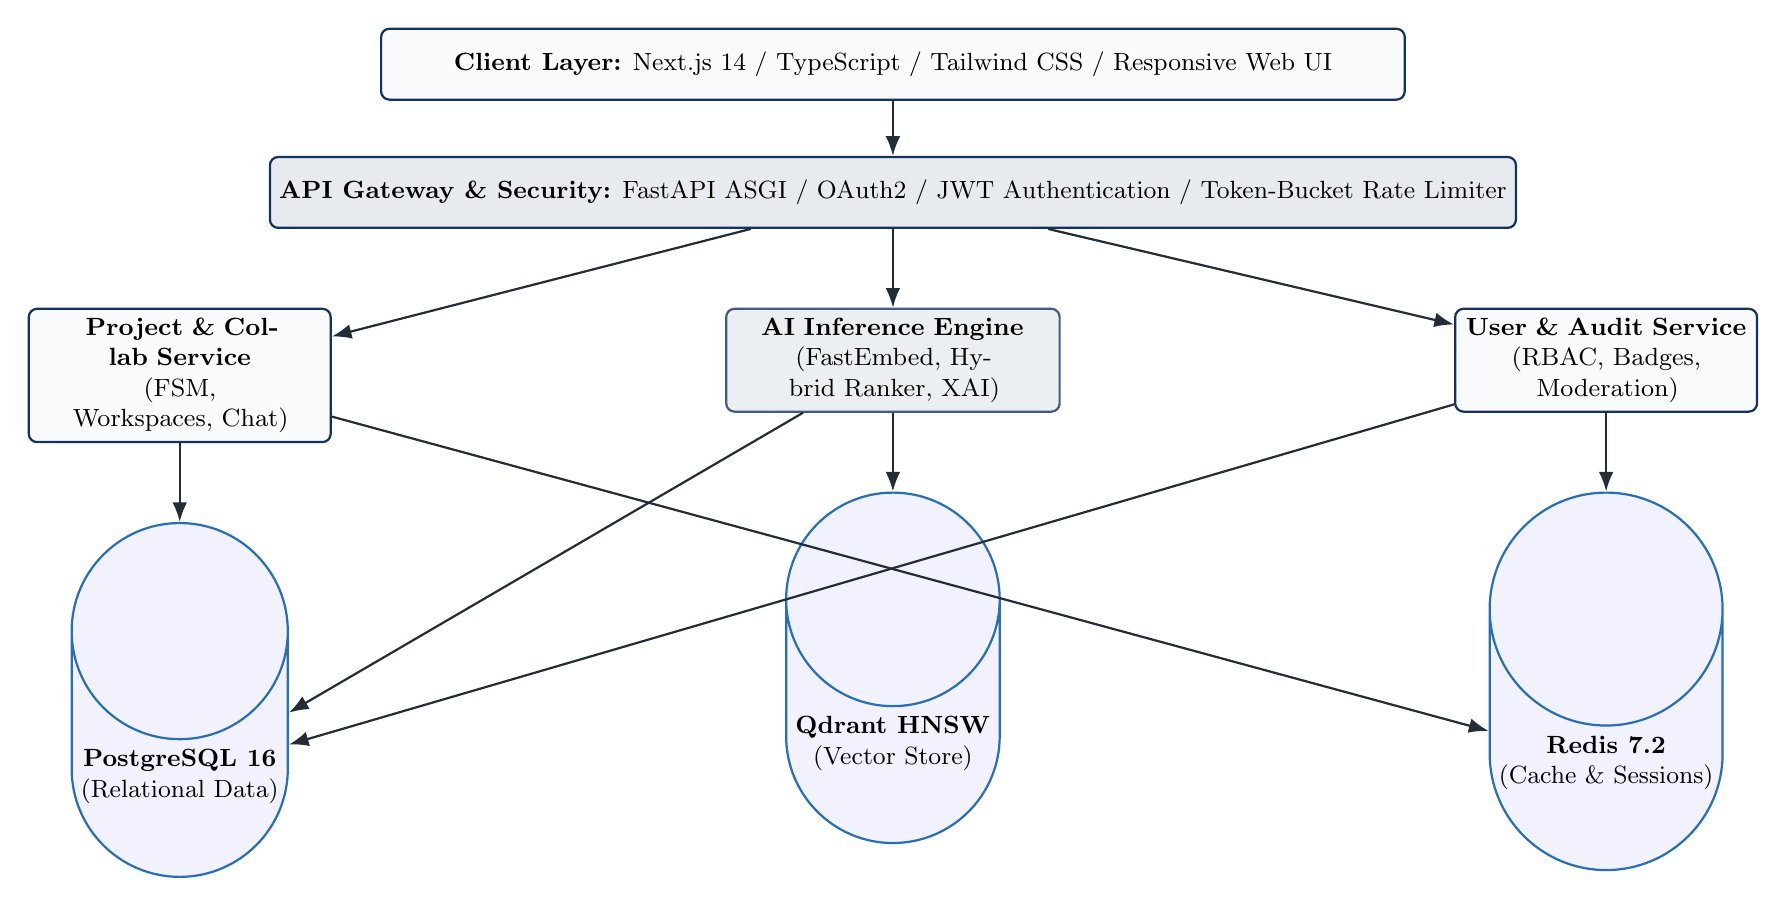
\begin{tikzpicture}[
    box/.style={rectangle, draw=primary, fill=lightbg, rounded corners=3pt, thick, align=center, font=\small, minimum height=0.9cm},
    databox/.style={cylinder, shape border rotate=90, draw=secondary, fill=blue!5, thick, align=center, font=\small, minimum height=1.0cm, minimum width=2.2cm},
    aibox/.style={rectangle, draw=primary!80, fill=primary!8, rounded corners=3pt, thick, align=center, font=\small, minimum height=0.9cm},
    arrow/.style={-{Latex[length=2.5mm]}, thick, color=darkslate}
]
    % Client
    \node[box, minimum width=13cm] (client) {\textbf{Client Layer:} Next.js 14 / TypeScript / Tailwind CSS / Responsive Web UI};

    % API Gateway
    \node[box, below=0.7cm of client, minimum width=13cm, fill=primary!10] (gateway) {\textbf{API Gateway \& Security:} FastAPI ASGI / OAuth2 / JWT Authentication / Token-Bucket Rate Limiter};

    % Microservices
    \node[box, below left=1.0cm and -0.8cm of gateway, text width=3.6cm] (projectsvc) {\textbf{Project \& Collab Service}\\(FSM, Workspaces, Chat)};
    \node[aibox, below=1.0cm of gateway, text width=4.0cm] (aisvc) {\textbf{AI Inference Engine}\\(FastEmbed, Hybrid Ranker, XAI)};
    \node[box, below right=1.0cm and -0.8cm of gateway, text width=3.6cm] (authsvc) {\textbf{User \& Audit Service}\\(RBAC, Badges, Moderation)};

    % Databases
    \node[databox, below=1.0cm of projectsvc] (postgres) {\textbf{PostgreSQL 16}\\(Relational Data)};
    \node[databox, below=1.0cm of aisvc] (vectordb) {\textbf{Qdrant HNSW}\\(Vector Store)};
    \node[databox, below=1.0cm of authsvc] (redis) {\textbf{Redis 7.2}\\(Cache \& Sessions)};

    % Connections
    \draw[arrow] (client) -- (gateway);
    \draw[arrow] (gateway) -- (projectsvc);
    \draw[arrow] (gateway) -- (aisvc);
    \draw[arrow] (gateway) -- (authsvc);

    \draw[arrow] (projectsvc) -- (postgres);
    \draw[arrow] (projectsvc) -- (redis);
    \draw[arrow] (aisvc) -- (vectordb);
    \draw[arrow] (aisvc) -- (postgres);
    \draw[arrow] (authsvc) -- (postgres);
    \draw[arrow] (authsvc) -- (redis);
\end{tikzpicture}%
}
\caption{UniExpert High-Level Architectural Topology}
\label{fig:architecture}
\end{figure}

\begin{table}[H]
\centering
\small
\caption{Selected Technology Stack and Justification}
\label{tab:tech_stack}
\begin{tabularx}{\textwidth}{@{}l l X@{}}
\toprule
\textbf{Layer} & \textbf{Technology} & \textbf{Architectural Rationale} \\
\midrule
Frontend Client & Next.js 14 / React & Server-side rendering, fast First Contentful Paint ($<1\text{s}$), responsive UI. \\
Backend Service & FastAPI (Python 3.11+) & High-throughput asynchronous ASGI web server; native Python ML integration. \\
Relational Storage & PostgreSQL 16 & ACID compliance, robust foreign key constraints, JSONB support for schemas. \\
Vector Database & Qdrant 1.8+ & High-performance Approximate Nearest Neighbor (ANN) search using HNSW indexing. \\
Embedding Model & \texttt{all-MiniLM-L6-v2} & 384-dimensional dense semantic vectors with sub-millisecond CPU inference latency. \\
In-Memory Store & Redis 7.2 & JWT session management, token blocklists, and rate-limiting buckets (60 req/min). \\
\bottomrule
\end{tabularx}
\end{table}

% ------------------------------------------------------------------------------
% 5. MOSCOW FEATURE SCOPE PRIORITIZATION
% ------------------------------------------------------------------------------
\section{Implementation Scope and MoSCoW Prioritization}

To guarantee successful delivery within the Fall 2026 12-week semester (October -- December 2026), project features are triaged using the MoSCoW framework in Table~\ref{tab:moscow}.

\begin{table}[H]
\centering
\small
\caption{MoSCoW Feature Prioritization for Fall 2026 Capstone}
\label{tab:moscow}
\begin{tabularx}{\textwidth}{@{}p{2.6cm} X p{3.2cm}@{}}
\toprule
\textbf{Priority} & \textbf{Feature Scope} & \textbf{Target Delivery} \\
\midrule
\textbf{Must-Have} \newline (Core MVP) & 
\begin{itemize}[leftmargin=*,noitemsep]
    \item Role-based authentication (Student, Expert, Admin) with email verification.
    \item Multi-tier expert credential verification (institutional badge Tiers 1--4).
    \item Natural language project statement submission and NLP skill extractor.
    \item Qdrant dense vector search with multi-criteria hybrid ranker (Eq.~\ref{eq:hybrid_matching}).
    \item Explainable AI (XAI) natural language justification generation.
    \item Collaboration request lifecycle Finite State Machine (FSM) and workspace.
\end{itemize} & \textbf{Oct -- Nov 2026} \newline (Weeks 1--8) \\
\addlinespace
\textbf{Should-Have} \newline (Extended Scope) & 
\begin{itemize}[leftmargin=*,noitemsep]
    \item Multidisciplinary problem decomposition and team builder (Eq.~\ref{eq:skill_gap}).
    \item Side-by-side candidate comparison matrix.
    \item Automated public Google Scholar / ORCID bibliometric synchronization.
    \item Post-collaboration double-blind mutual peer reviews.
\end{itemize} & \textbf{December 2026} \newline (Weeks 9--12) \\
\addlinespace
\textbf{Could-Have} \newline (Future Work) & Real-time WebRTC audio/video rooms, cross-institutional federation, mobile apps. & Post-Capstone \\
\bottomrule
\end{tabularx}
\end{table}

% ------------------------------------------------------------------------------
% 6. TIMELINE & MILESTONES
% ------------------------------------------------------------------------------
\section{Semester Development Plan and Milestones (Fall 2026)}

The 12-week execution schedule spans October through December 2026 across three defined monthly milestones, as detailed in Table~\ref{tab:timeline}.

\begin{table}[H]
\centering
\small
\caption{Fall 2026 Capstone Execution Timeline and Milestone Deliverables}
\label{tab:timeline}
\begin{tabularx}{\textwidth}{@{}p{2.4cm} p{1.8cm} X p{3.2cm}@{}}
\toprule
\textbf{Phase} & \textbf{Weeks} & \textbf{Key Deliverables \& Activities} & \textbf{Milestone} \\
\midrule
\textbf{Month 1} \newline (October 2026) & Weeks 1--4 & 
\begin{itemize}[leftmargin=*,noitemsep]
    \item Requirements elicitation and formal IEEE 830 SRS documentation.
    \item Literature review on expert finding systems and vector search.
    \item Database schema design (PostgreSQL), API contracts, and CI/CD setup.
\end{itemize} & \textbf{M1: System Blueprint} \newline (Requirements \& Design) \\
\addlinespace
\textbf{Month 2} \newline (November 2026) & Weeks 5--8 & 
\begin{itemize}[leftmargin=*,noitemsep]
    \item Implement OAuth2/JWT authentication and profile verification services.
    \item Build NLP skill extraction pipeline and integrate Qdrant vector database.
    \item Deploy hybrid multi-criteria ranking engine and collaboration FSM.
\end{itemize} & \textbf{M2: Core Platform} \newline (Functional Matchmaker) \\
\addlinespace
\textbf{Month 3} \newline (December 2026) & Weeks 9--12 & 
\begin{itemize}[leftmargin=*,noitemsep]
    \item Multidisciplinary team builder and skill gap optimizer.
    \item Empirical IR benchmarking (BM25 vs. Vector vs. Hybrid: Precision@K, NDCG@K).
    \item User Acceptance Testing (UAT), comprehensive report, and final defense.
\end{itemize} & \textbf{M3: Final Defense} \newline (Evaluation \& Sign-Off) \\
\bottomrule
\end{tabularx}
\end{table}

% ------------------------------------------------------------------------------
% 7. RISK MITIGATION & EXPECTED OUTCOMES
% ------------------------------------------------------------------------------
\section{Risk Management and Expected Capstone Outcomes}

\begin{table}[H]
\centering
\small
\caption{Project Risk Matrix and Engineered Mitigations}
\label{tab:risks}
\begin{tabularx}{\textwidth}{@{}p{3.0cm} c c X@{}}
\toprule
\textbf{Identified Risk} & \textbf{Likelihood} & \textbf{Impact} & \textbf{Engineered Mitigation Protocol} \\
\midrule
Profile Cold-Start & High & High & Pre-seed database with public faculty profiles; enable automated ORCID sync. \\
Vector Search Latency & Low & High & Pre-compute embeddings; utilize HNSW indexing; cache top domain queries in Redis. \\
Credential Falsification & Med & High & Enforce \texttt{.edu} email verification; require admin review for Tier 3 faculty badges. \\
Faculty Availability Fatigue & High & Med & Monthly request quotas (max 5 pending); calendar blackout toggles. \\
\bottomrule
\end{tabularx}
\end{table}

\subsection{Expected Capstone Outcomes}
Upon completion in December 2026, UniExpert will deliver:
\begin{enumerate}[noitemsep]
    \item A production-grade, accessible web platform conforming to modern software engineering standards.
    \item An empirical benchmarking evaluation proving statistically significant improvements in recommendation accuracy ($NDCG@5$, Precision@5) over classical keyword and pure vector baselines.
    \item A formal capstone thesis documentation package prepared for university repository archiving.
\end{enumerate}

\end{document}
